\chapter{PENGUJIAN DAN ANALISA}
\vspace{1ex}

\section*{}
Pada bab ini dipaparkan hasil pengujian dari Tugas Akhir serta analisa dari desaim sistem simulator dan implementasinya. Pengujian dibagi menjadi lima bagian antara lain:
\vspace{1ex}
\begin{enumerate}[nolistsep]
	\item Pengujian \textit{User Interface} - Pemilihan Jumlah Lajur
	\item Pengujian Pengambilan Data - Kecepatan
	\item Pengujian Pengambilan Data - Informasi Spasial
	\item Pengujian Pengambilan Data - \textit{Response Time} dan \textit{Input} Pengemudi
	\item Pengujian Pengambilan Data - Citra \textit{Webcam}
	\item Pengujian Pengambilan Data - \textit{Serial Data USB}
	\item Pengujian Respon Sinyal dari \textit{Steering Wheel Controller} terhadap simulator
	\item Pengujian \textit{User Experience} / UX Pengguna
	
	\vspace{1ex}

\end{enumerate}
Dengan dilaksanakannya beberapa pengujian tersebut, sehingga dapat ditarik kesimpulan dari pelaksanaan tugas akhir ini.
\vspace{1ex}

\section{Pengujian \textit{User Interface} - Pemilihan Jumlah Lajur}
\vspace{1ex}

Pada pengujian \textit{user interface}, \textit{user} dapat memilih jumlah lajur yang akan digunakan. Terdapat 4 \textit{scene} yang dapat dipilih dari \textit{user interface}, yaitu 2 lajur (pendek), 2 lajur (panjang) , 3 lajur, serta 4 lajur.

Kesimpulan pada pengujian \textit{user interface} (Gambar \ref{fig:4.1}), tombol menu lajur yang ditampilkan dan yang dipilih oleh \textit{user} sudah berkorelasi dengan \textit{scene} yang dimuat oleh game.

\section{Pengujian Pengambilan Data - Kecepatan}
\vspace{1ex}

Pada pengujian pengambilan data kecepatan, didapatkan data seperti pada tabel \ref{tb:4_2}, data yang didapatkan merupakan data mentah \textit{(raw data)} tanpa pengolahan atau kalkulasi tambahan, dari \textit{Unity Game Engine} dengan cara mengakses komponen \textit{RigidBody Game Object} mobil, dengan fungsi \texttt{GetComponent<Rigidbody>()}, sehingga didapatkan \textit{object variable} yaitu \texttt{velocity} untuk mendapatkan kecepatan vektor \textit{x,y,z}, serta \texttt{velocity.magnitude} untuk mendapatkan besaran dari kecepatan vektor tersebut. Pengambilan / \textit{sampling} data dilakukan tiap frame, sehingga tabel \ref{tb:4_2} hanya menampilkan data kurang lebih $\frac{1}{2}$ detik.

Dapat disimpulkan pengujian ini (tabel \ref{tb:4_2}) dapat menghasilkan data dengan tingkat akurasi yang tinggi, dikarenakan data dapat diambil dalam rentang waktu yang cukup kecil tiap framenya (Unit tiap Frame).

\section{Pengujian Pengambilan Data - Informasi Spasial}
\vspace{1ex}

Informasi spasial pada pengujian ini terdapat 2 macam data, yaitu posisi relatif kendaraan terhadap jalan, serta sudut orientasi kendaraan. Data posisi relatif terhadap jalan didapat dari mengukur jarak terdekat dari titik pusat masa kendaraan ke garis batas lajur kanan dan garis batas lajur kiri, dengan mengakses salah satu \textit{object} dari \textit{Bézier Path Creator}\cite{cit:16} \texttt{PathCreator.path} sehingga didapatkan \textit{object method} \texttt{GetClosestPointOnPath()} untuk mendapatkan koordinat terdekat dari mobil dari class tersebut, lalu akses class \textit{transform} dari \textit{game object} mobil, untuk mendapatkan koordinat dari \textit{center of mass} mobil simulator menggunakan \texttt{transform.position}, kemudian setelah didapatkan 2 koordinat yang ingin  diukur jaraknya, sehingga kemudian dapat menggunakan fungsi dari \textit{unity} yaitu \texttt{Vector3.Distance()} untuk mendapatkan jarak dari kedua koordinat tersebut. 

\par Kemudian Sudut Orientasi kendaraan pada pengujian ini menggunakan  Sudut spasial \textit{Euler} untuk mengetahui orientasi kendaraan pada 3 dimensi,  untuk mendapatkan nilai tersebut pada \textit{unity},  \textit{script} dapat mengakses \textit{class variable} \texttt{transform.eulerAngles}. 

\par  Maka dari itu, untuk posisi relatif, terdapat 2 macam data yaitu, Jarak dari batas kanan dan Jarak dari batas kiri dengan cara mengukur jarak dari 2 koordinat yaitu, \textit{center of mass} mobil dan titik terdekat dari \textit{center of mass} tersebut, sedangkan untuk Sudut Orientasi kendaraan, didapatkan 3 macam data yaitu, sudut orientasi relatif terhadap sumbu \textit{x,y,z} atau \textit{6 Degree of Freedom - Pitch, Yaw, and Roll}. Berikut datanya pada tabel \ref{tb:4_3}

Kesimpulan yang dapat ditarik pada pengujian pengambilan data informasi spasial adalah, pada tabel \ref{tb:4_3}, dapat diketahui bahwa lebar dari jalan pada simulator adalah kurang lebih 12 unit, dengan menggunakan 2 data tersebut, yaitu jarak mobil dari batas kiri dan kanan jalan, sehingga dapat diketahui lokasi tepatnya dari mobil. Selain itu, dapat disimpulkan juga bahwa mobil berada di jalan yang datar, dikarenakan nilai sudut \textit{euler} dari sumbu \textit{x} dan sumbu \textit{z} mendekati 0.

\section{Pengujian Pengambilan Data - \textit{Response Time} dan \textit{Input} Pengemudi}
\vspace{1ex}

\textit{Response Time} adalah waktu yang menunjukkan seberapa secepat pengemudi kembali ke lajur semula apabila simulator telah mendeteksi mobil keluar dari lajur sebelah kiri. Durasi yang dihitung adalah semenjak mobil keluar dari lajur, hingga mobil kembali ke lajur. Data yang didapat dari simulator berupa waktu dalam sekon, serta durasi frame semenjak mobil keluar dari lajur.

Selain itu diperlukannya perubahan definisi dari 'keluar jalur' apabila sistem mendeteksi bahwa pengemudi akan menyalip kendaraan yang lain. Pada kasus tersebut, pendeteksian keluar jalur akan diberikan \textit{flag} bahwasanya terdapat mobil didepan kendaraan pengemudi, sehingga pendeteksian sistem keluar jalur sementara dimatikan. Apabila sistem sudah mendeteksi tidak ada kendaraan didepan pengemudi, sistem pendeteksian keluar jalur akan berjalan kembali.

Kemudian, pada pengujian ini erat kaitannya dengan mendeteksi respon \textit{input} dari pengemudi. Maka dari itu, informasi \textit{input} dari pengemudi juga perlu di lakukan pengambilan datanya agar diketahui sudut dari \textit{steering wheel} serta tekanan pedal gas dan rem. Data - data \textit{input}ini penting dikarenakan berkaitan dengan data respon pengemudi ketika pengemudi mengetahui adanya rintangan atau objek tidak terduga ketika di jalan. Dengan menganalisa grafik sudut \textit{steering wheel} dan tekanan pedal gas dan rem, akan didapatkan redundansi data selain citra wajah pengemudi serta data - data biometrik pengemudi seperti EEG dan ECG, untuk analisa proses kapan terjadinya \textit{microsleep} pada pengemudi. Grafik data \textit{input} dari pengemudi bisa di lihat pada gambar \ref{fig:4.5}

\section{Pengujian Pengambilan Data - \textit{Citra Webcam}}
\vspace{1ex}

Pada gambar \ref{fig:4.2}, bisa dilihat hasil dari \textit{capture webcam} yang telah di \textit{encode} menjadi format \textit{.png}. 
\par Kesimpulan dari pengujian pengambilan data \textit{webcam} ini menunjukkan bahwa, harus dipastikan bahwa \textit{source} dari \textit{webcam} telah tepat terdeteksi sebagai suatu alat pengambil citra pada unity. Kemudian dipastikan apakah hasil \textit{encode} telah menghasilkan keluaran gambar yang diinginkan. Terjadinya kesalahan pendeteksian \textit{camera source} atau terjadinya kesalahan pada proses \textit{encode}, akan menyebabkan hasil keluaran citra \textit{webcam} tidak sesuai dengan yang diharapkan.

\section{Pengujian Pengambilan Data - \textit{Serial Data USB}}
\vspace{1ex}

\textit{Serial Data} disini ialah, data yang didapatkan dari komunikasi via \textit{serial USB}. Desain sistem komunikasi serial menggunakan port COM, bisa dilihat pada gambar \ref{tb:4_3}. 
\par Pada tugas akhir ini, sistem komunikasi serial arduino dengan - PC simulator adalah menggunakan script python untuk mengakses \textit{Port COM} yang menghubungkan Arduino dengan PC. Setelah \textit{Port COM} Diakses oleh script python, script python akan menerima \textit{byte} data dari Arduino, kemudian script tersebut akan merubah data menjadi angka bilangan bulat atau \textit{integer} tiap 4 \textit{byte (32 bit)} data yang masuk.
\par Kemudian setelah data dirubah menjadi data angka bilangan bulat, script python akan mengakses \textit{file system} dari komputer, dan akan membuat file dengan ekstensi \textit{.csv}, lalu menambahkan angka tersebut kedalam file yang baru dibuat tersebut, serta memformat dengan \textit{column separator ' \textbackslash{}t '} dan \textit{row separator ' \textbackslash{}n '}.

\section{Pengujian Respon Sinyal dari \textit{Steering Wheel Controller} terhadap simulator}
\vspace{1ex}

Pada pengujian ini, dikarenakan sistem memiliki mekanisme masukan dari pengguna berupa \textit{steering wheel controller}, maka diperlukan pengujian respon dari \textit{steering wheel controller} terhadap proses - proses berjalan di \textit{unity}. Kegiatan pengujian adalah dengan membandingkan sinyal dari \textit{steering wheel controller} yang berjalan sebelum \textit{script - script} lain pada unity, dengan sinyal yang setelah melalui proses - proses / \textit{script} lain pada unity. Hal ini dapat dilakukan dengan menerapkan fitur \textit{Script Execution Order} pada unity.
Grafik data sinyal tersebut bisa dilihat pada gambar \ref{fig:4.6} dan \ref{fig:4.7}, sedangkan grafik analisa \textit{error} kuantitatif nilai error bisa dilihat pada gambar \ref{fig:4.8}
\par Dari analisa kuantitaf terhadap nilai error tersebut, dapat dilihat bahwa grafik nilai error selalu mendekati 0 persen ketika \textit{runtime}, sehingga dapat disimpulkan bahwa \textit{input} dari \textit{steering wheel} tidak terlalu terpengaruh proses yang berjalan pada unity, sehingga grafik terlihat saling menindih.

\section{Pengujian \textit{User Experience} / UX dari Pengguna}
\vspace{1ex}

Pengujian kepuasan pengguna dilakukan dengan melakukan pengujian terhadap subjek pengendara mobil kemudian dilakukan proses pengisian kuesioner setelah pengguna mencoba alat simulator. Jumlah responden dalam pengujian kepuasan pengguna ini sebanyak 3 responden, terdiri dari keluarga dekat penulis. Hal ini dikarenakan keterbatasan situasi dan kondisi dimana ketika pengujian dilakukan sedang adanya pandemi \textit{COVID-19}, sehingga hal tersebut membatasi jumlah responden yang bersukarela mencoba alat simulator ini. Responden menerima 17 buah pernyataan sesuai pada tabel \ref{tb:4_7} Opsi tingkat persetujuan yang disediakan adalah sebagai berikut :

    \begin{enumerate}[nolistsep]
	\item Sangat Tidak Setuju (STS)
	\item Tidak Setuju (TS)
	\item Netral (N)
	\item Setuju (S)
	\item Sangat Setuju (SS)
	
	\vspace{1ex}
\end{enumerate}

%Daftar pertanyaan kuesioner UX
\begin{table}[]
\caption{Skenario kuesioner untuk pengujian kepuasan pengguna}
\label{tb:4_7}
\begin{tabular}{|c|p{9.5cm}|}
\hline
\textbf{No} & \multicolumn{1}{c|}{\textbf{Pertanyaan}}                                                                         \\ \hline
1           & Saya mengetahui tentang teknologi simulasi                                                                       \\ \hline
2           & Saya mengetahui tentang game yang melibatkan mengendarai mobil                                                   \\ \hline
3           & Saya pernah mengemudikan mobil virtual (game, simulator sim, dll)                                                \\ \hline
4           & Saya merasa menu User Interface Pemilihan Jumlah lajur aplikasi simulator   sudah jelas                          \\ \hline
5           & Saya merasa menu User Interface Pemilihan Jumlah lajur aplikasi simulator   sudah menarik                        \\ \hline
6           & Saya merasa user interface dashboard mobil sudah jelas                                                           \\ \hline
7           & Saya merasa user interface dashboard mobil sudah menarik                                                         \\ \hline
8           & Saya merasa user interface tutorial cara mengemudikan mobil sudah jelas                                          \\ \hline
9           & Saya merasa penggunaan perangkat keras steering wheel controller sudah   intuitif                                \\ \hline
10          & Saya merasa jumlah lajur yang yang dapat dipilih sudah mewakili berbagai   macam kondisi jalan yang sesungguhnya \\ \hline
11          & Saya merasa simulasi yang disajikan sudah cukup realistis                                                        \\ \hline
12          & Saya merasa pemandangan yang disediakan pada tiap - tiap lajur sudah   cukup menarik                             \\ \hline
13          & Saya merasa tertarik akan teknologi simulasi berkendara untuk riset                                              \\ \hline
14          & Saya merasa teknologi simulasi dapat menggantikan proses pengambilan data   di lapangan                          \\ \hline
15          & Saya menjadi tertarik untuk menggunakan simulator ini                                                            \\ \hline
16          & Saya setuju perangkat ini untuk diterapkan di institusi penelitian di   Indonesia                                \\ \hline
17          & Saya setuju perangkat ini dapat mendukung perkembangan riset deteksi   pengemudi mengantuk                       \\ \hline
\end{tabular}
\end{table}

Terdapat 3 macam pertanyaan yang diajukan, yaitu pertanyaan dengan tujuan untuk mengetahui bagaimana pengetahuan pengguna tentang teknologi simulasi khususnya teknogi simulasi berkendara, pertanyaan dengan tujuan untuk mengukur bagaimana kepuasan pengguna terhadap tampilan serta realitas simulasi, serta yang terakhir pertanyaan dengan tujuan untuk mengetahui bagaimana pendapat pengguna tentang teknologi simulator yang diterapkan untuk proses pengambilan data di lapangan.
\par Pengujian kepuasan pengguna dihitung dari banyaknya presentase total poin yang didapatkan dari total maksimal poin untuk setiap pernyataan yang disediakan (likert scale). Berdasarkan parameter tersebut, setiap opsi memiliki poin yang berbeda yaitu SS=5 poin, S=4 poin, N=3 poin, TS=2 poin, dan STS=1 poin. Semakin besar presentasenya, maka semakin \textit{valid} pernyataan tersebut. 
\par Berikut hasil dari proses pengujian tingkat kepuasan pengguna (tabel \ref{tb:4_8})

\begin{table}[]
\caption{Hasil pengujian kepuasan pengguna.}
\label{tb:4_8}
\begin{tabular}{|c|l|l|l|l|l|}
\hline
\multirow{2}{*}{\textbf{Pernyataan}} & \multicolumn{5}{c|}{\textbf{Jawaban}}                                                                                                                                       \\ \cline{2-6} 
                                     & \multicolumn{1}{c|}{\textbf{STS}} & \multicolumn{1}{c|}{\textbf{TS}} & \multicolumn{1}{c|}{\textbf{N}} & \multicolumn{1}{c|}{\textbf{S}} & \multicolumn{1}{c|}{\textbf{SS}} \\ \hline
Pernyataan 1                         & 0,00\%                            & 0,00\%                           & 0,00\%                          & 66,67\%                         & 33,33\%                          \\ \hline
Pernyataan 2                         & 33,33\%                           & 0,00\%                           & 0,00\%                          & 33,33\%                         & 33,33\%                          \\ \hline
Pernyataan 3                         & 33,33\%                           & 0,00\%                           & 0,00\%                          & 33,33\%                         & 33,33\%                          \\ \hline
Pernyataan 4                         & 0,00\%                            & 0,00\%                           & 33,33\%                         & 33,33\%                         & 33,33\%                          \\ \hline
Pernyataan 5                         & 0,00\%                            & 0,00\%                           & 0,00\%                          & 100,00\%                        & 0,00\%                           \\ \hline
Pernyataan 6                         & 0,00\%                            & 0,00\%                           & 33,33\%                         & 33,33\%                         & 33,33\%                          \\ \hline
Pernyataan 7                         & 0,00\%                            & 0,00\%                           & 33,33\%                         & 66,67\%                         & 0,00\%                           \\ \hline
Pernyataan 8                         & 0,00\%                            & 0,00\%                           & 0,00\%                          & 33,33\%                         & 66,67\%                          \\ \hline
Pernyataan 9                         & 0,00\%                            & 0,00\%                           & 100,00\%                        & 0,00\%                          & 0,00\%                           \\ \hline
Pernyataan 10                        & 0,00\%                            & 0,00\%                           & 33,33\%                         & 33,33\%                         & 33,33\%                          \\ \hline
Pernyataan 11                        & 0,00\%                            & 0,00\%                           & 0,00\%                          & 33,33\%                         & 66,67\%                          \\ \hline
Pernyataan 12                        & 0,00\%                            & 0,00\%                           & 33,33\%                         & 33,33\%                         & 33,33\%                          \\ \hline
Pernyataan 13                        & 0,00\%                            & 0,00\%                           & 0,00\%                          & 33,33\%                         & 66,67\%                          \\ \hline
Pernyataan 14                        & 0,00\%                            & 0,00\%                           & 33,33\%                         & 33,33\%                         & 33,33\%                          \\ \hline
Pernyataan 15                        & 0,00\%                            & 0,00\%                           & 66,67\%                         & 0,00\%                          & 33,33\%                          \\ \hline
Pernyataan 16                        & 0,00\%                            & 0,00\%                           & 0,00\%                          & 33,33\%                         & 66,67\%                          \\ \hline
Pernyataan 17                        & 0,00\%                            & 0,00\%                           & 0,00\%                          & 33,33\%                         & 66,67\%                          \\ \hline
\end{tabular}
\end{table}

% GAMBAR USER INTERFACE
\begin{figure} [!htb]
	\captionsetup{justification=centering}
	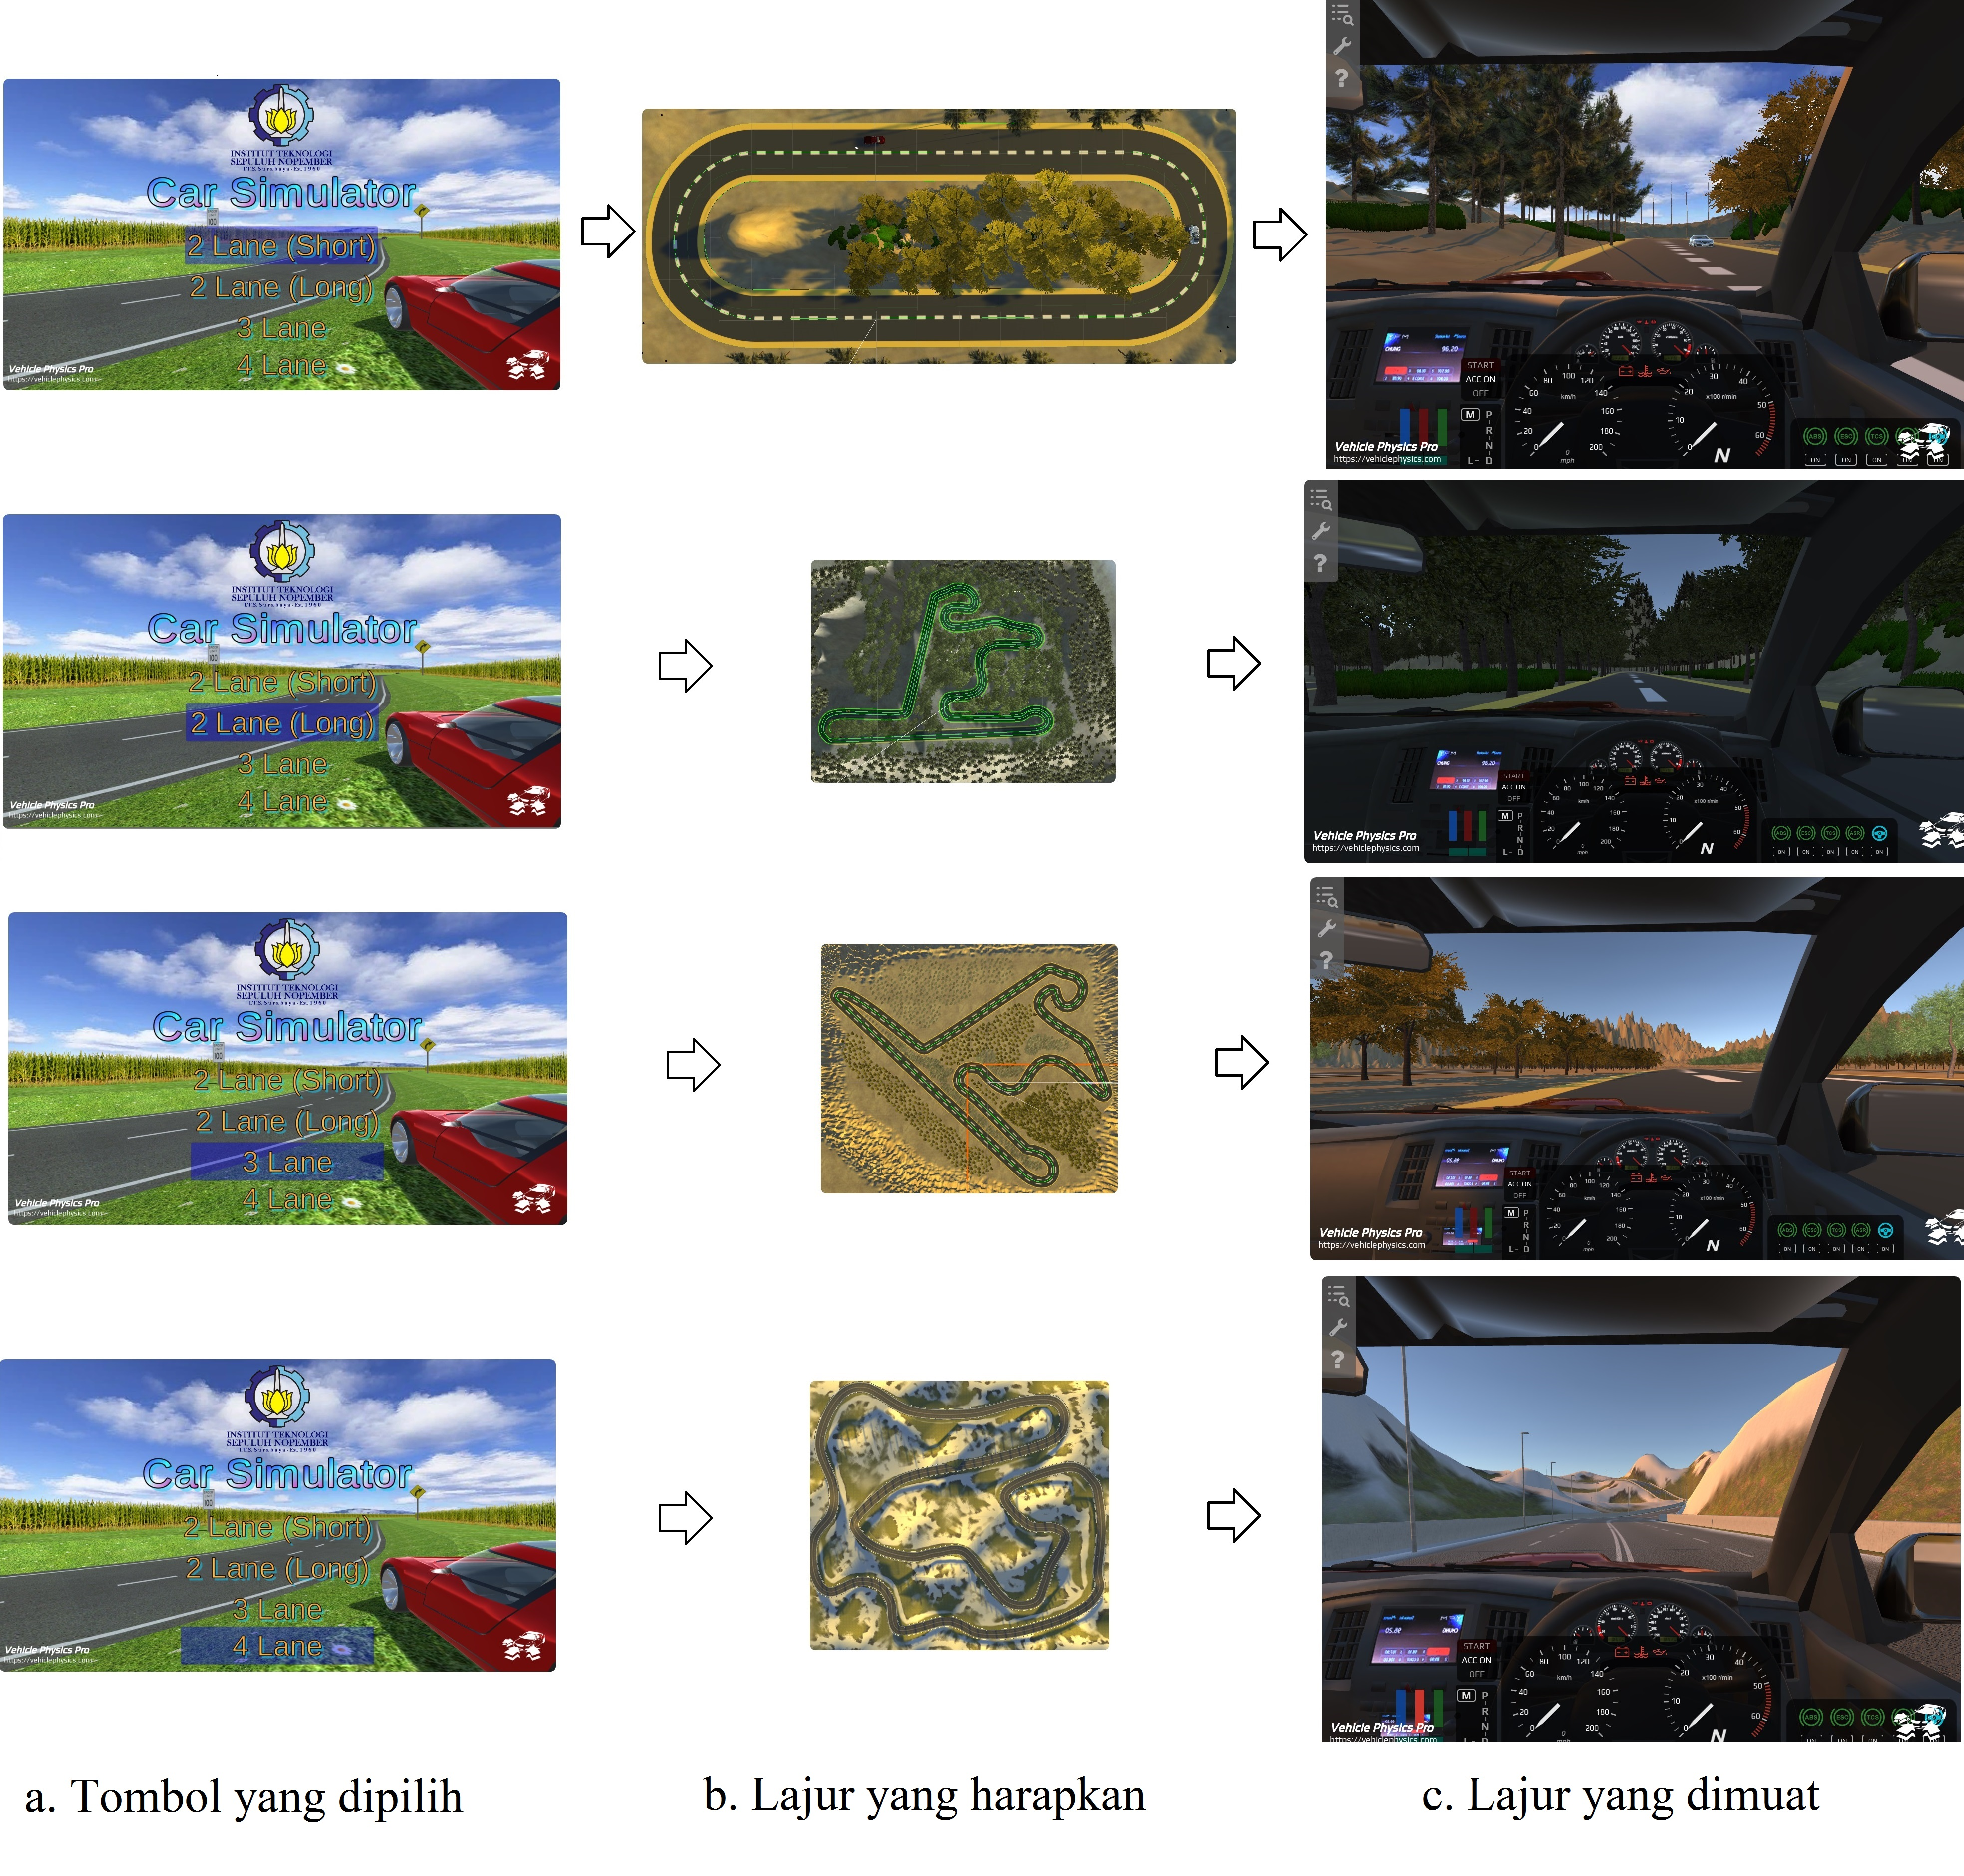
\includegraphics[scale=0.1]{img/UItest.jpg}
	\caption{Korelasi \textit{user interface} pemilihan lajur dengan \textit{scene} yang dimuat oleh simulator}
	\label{fig:4.1}
\end{figure}

%DATA SCREENSHOT WEBCAM
\begin{figure} [!htb]
	\captionsetup{justification=centering}
	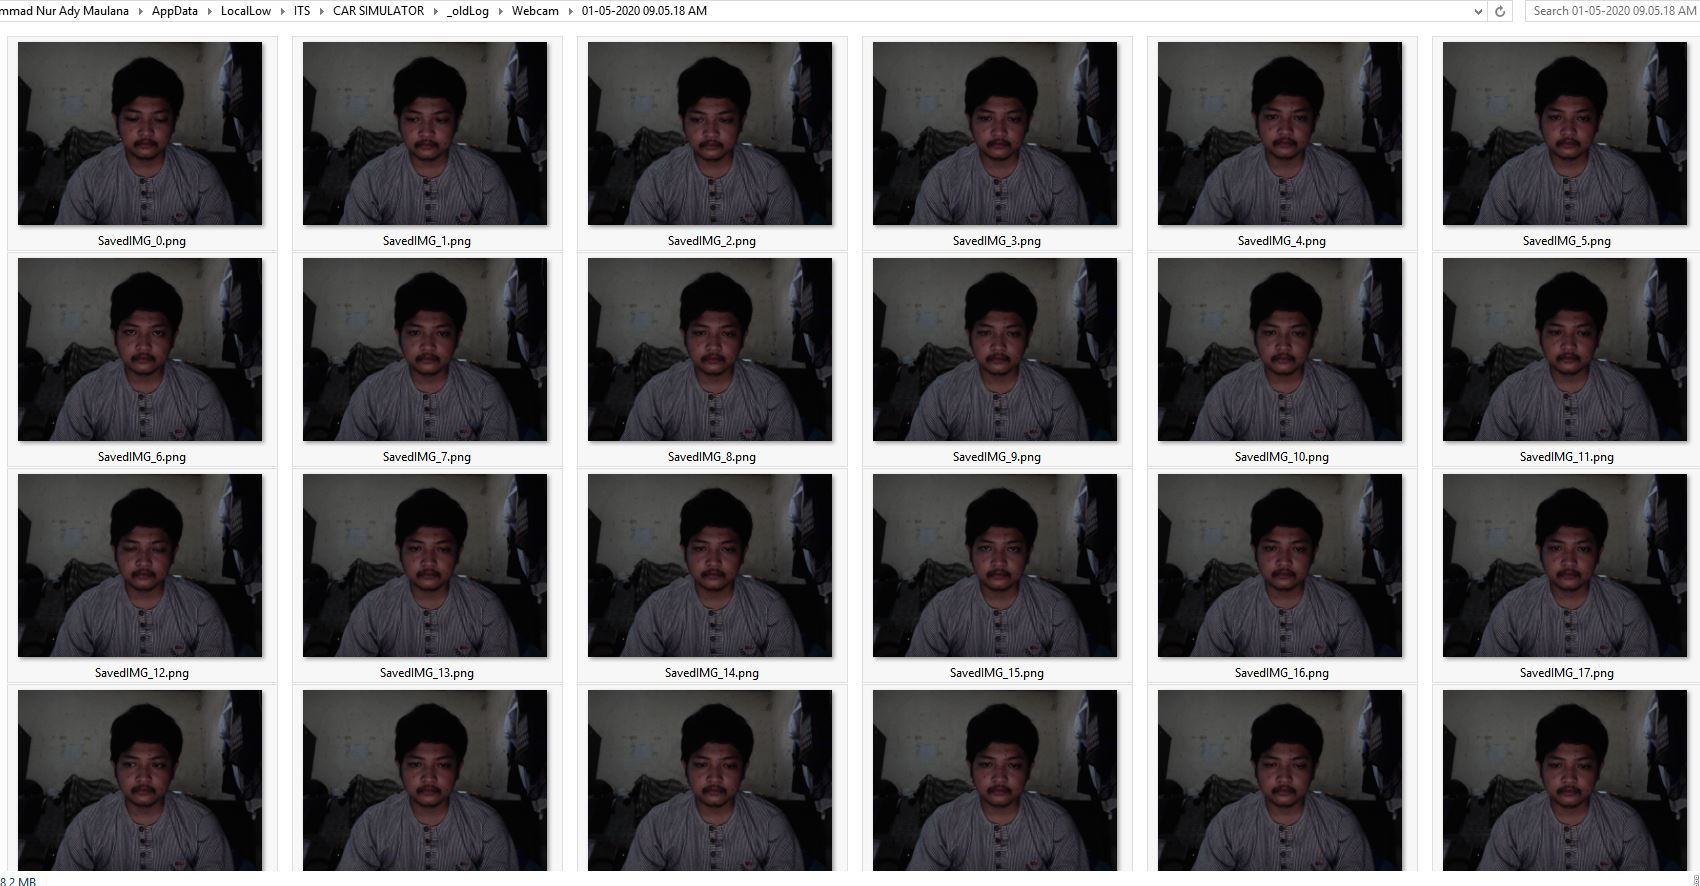
\includegraphics[scale=0.23]{img/webcam.JPG}
	\caption{\textit{Frame webcam} yang tersimpan di dalam \textit{harddrive}}
	\label{fig:4.2}
\end{figure}

%DATA GRAFIK SENSOR SERIAL
\begin{figure} [!htb]
	\captionsetup{justification=centering}
	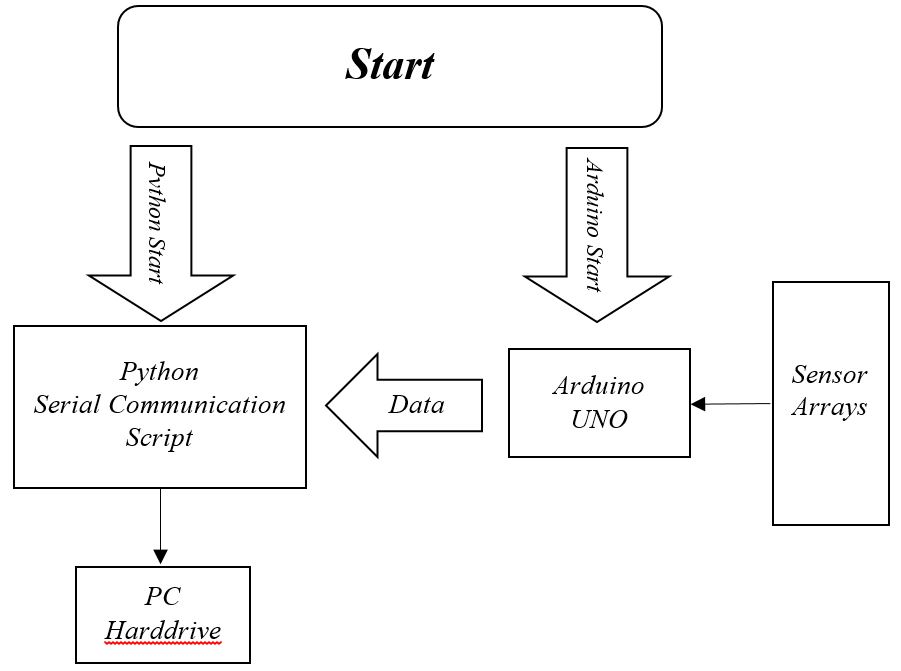
\includegraphics[scale=0.4]{img/arduino-python.JPG}
	\caption{Diagram Sistem Komunikasi Arduino Dengan PC Simulator}
	\label{fig:4.3}
\end{figure}

\begin{figure} [!htb]
	\captionsetup{justification=centering}
	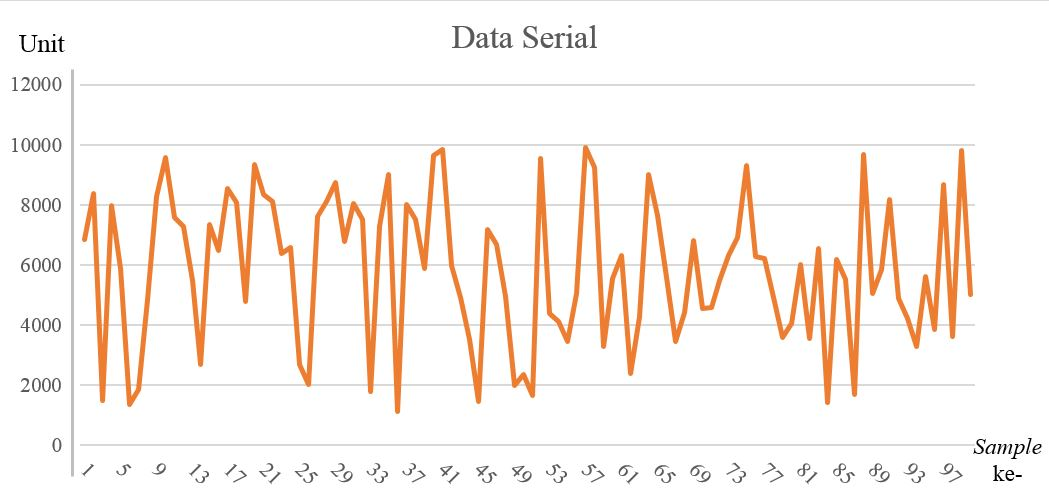
\includegraphics[scale=0.4]{img/serial.JPG}
	\caption{Contoh data serial yang diterima oleh arduino}
	\label{fig:4.4}
\end{figure}

\begin{figure} [!htb]
	\captionsetup{justification=centering}
	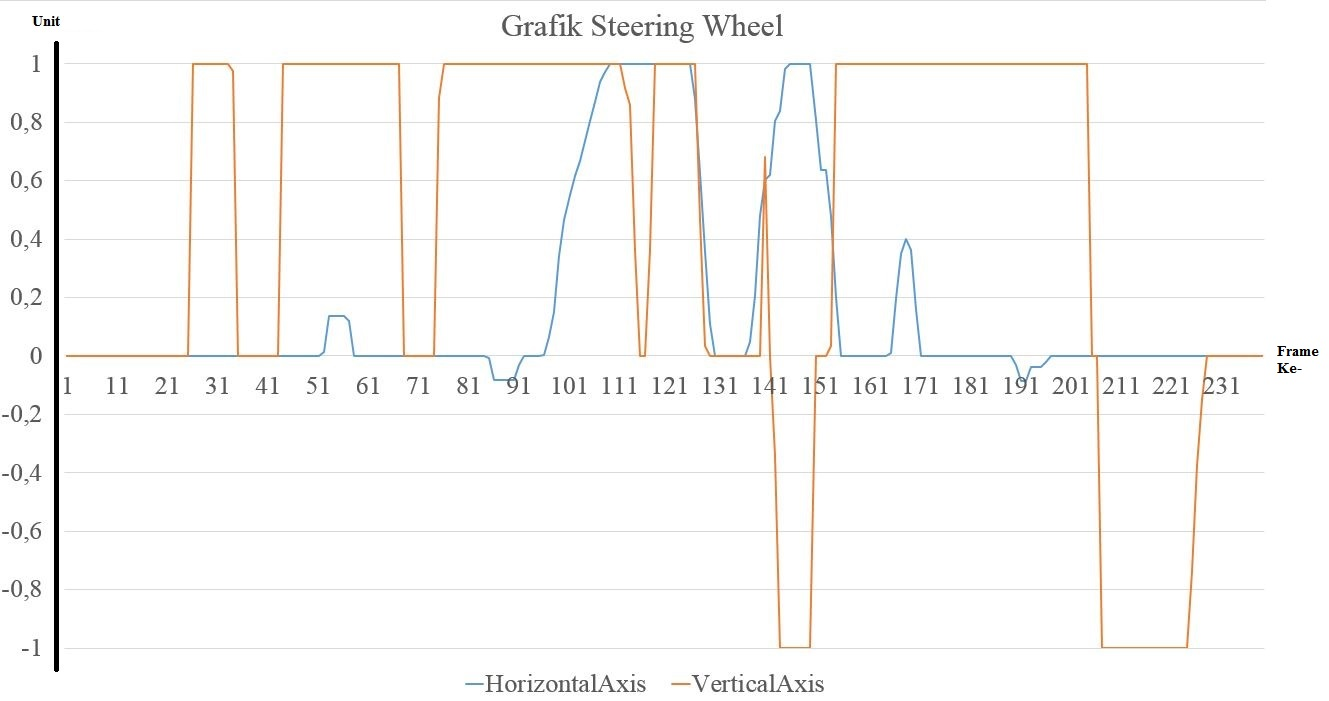
\includegraphics[scale=0.3]{img/driverinput.JPG}
	\caption{\textit{Input} dari pengemudi - \textit{Horizontal Axis} adalah Data sudut \textit{steering wheel}, \textit{Vertical Axis} adalah data nilai tekanan pedal gas / rem}
	\label{fig:4.5}
\end{figure}

\begin{figure} [!htb]
	\captionsetup{justification=centering}
	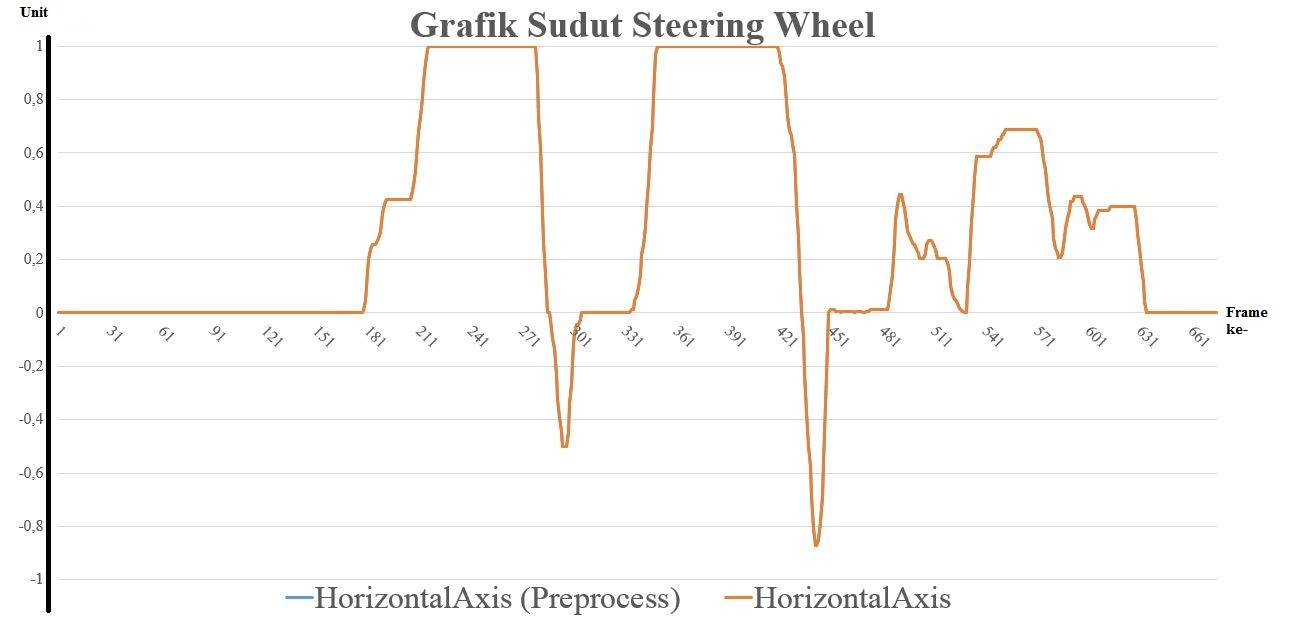
\includegraphics[scale=0.3]{img/response_horz.JPG}
	\caption{Perbandingan sinyal dari \textit{steering wheel controller}, sebelum dan sesudah grafik unity - \textit{Horizontal Axis} / Sudut \textit{steering wheel}}
	\label{fig:4.6}
\end{figure}

\begin{figure} [!htb]
	\captionsetup{justification=centering}
	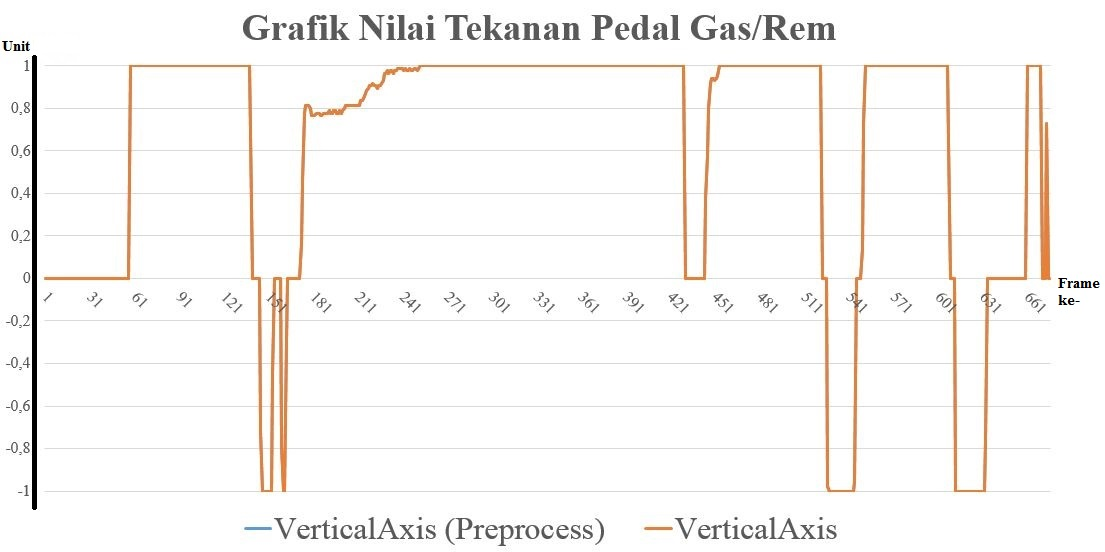
\includegraphics[scale=0.3]{img/response_vert.JPG}
	\caption{Perbandingan sinyal dari \textit{steering wheel controller}, sebelum dan sesudah grafik unity - \textit{Vertical Axis} / Nilai tekanan pedal gas/rem}
	\label{fig:4.7}
\end{figure}

\begin{figure} [!htb]
	\captionsetup{justification=centering}
	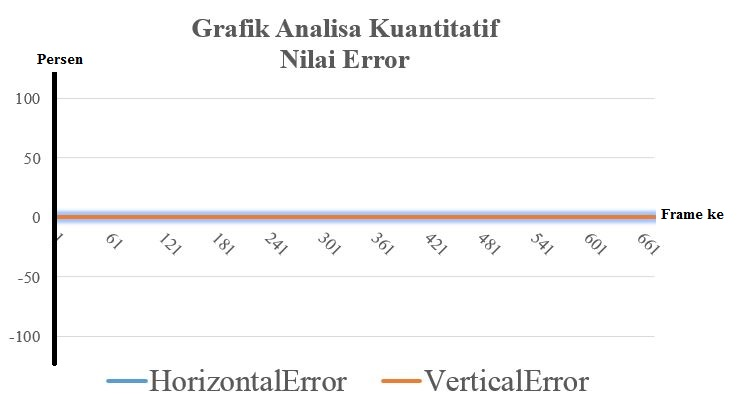
\includegraphics[scale=0.6]{img/grafik-error.JPG}
	\caption{Grafik analisa kuantitatif nilai error dari \textit{steering wheel controller}}
	\label{fig:4.8}
\end{figure}

% TABEL INPUT PENGEMUDI
\begin{table}[]
\caption{Tabel \textit{Input} Pengemudi Selama Kurang Lebih 1 Detik}
\label{tb:4_6}
\begin{tabular}{|c|c|c|c|}
\hline
\textit{\textbf{HorizontalAxis}} & \textit{\textbf{VerticalAxis}} & \textit{\textbf{Frame}} & \textit{\textbf{DateTime}} \\ \hline
0                                & 0                              & 74                      & 01.22.25.590387            \\ \hline
0                                & 0,8822352                      & 75                      & 01.22.25.748759            \\ \hline
0                                & 1                              & 76                      & 01.22.25.923766            \\ \hline
0                                & 1                              & 77                      & 01.22.26.234632            \\ \hline
0                                & 1                              & 78                      & 01.22.26.413535            \\ \hline
0                                & 1                              & 79                      & 01.22.26.570931            \\ \hline
0                                & 1                              & 80                      & 01.22.26.736147            \\ \hline
0                                & 1                              & 81                      & 01.22.26.892566            \\ \hline
0                                & 1                              & 82                      & 01.22.27.071471            \\ \hline
0                                & 1                              & 83                      & 01.22.27.225934            \\ \hline
0                                & 1                              & 84                      & 01.22.27.390172            \\ \hline
-0,007369441                     & 1                              & 85                      & 01.22.27.574942            \\ \hline
-0,08203134                      & 1                              & 86                      & 01.22.27.756776            \\ \hline
-0,08203134                      & 1                              & 87                      & 01.22.27.921995            \\ \hline
-0,08203134                      & 1                              & 88                      & 01.22.28.186928            \\ \hline
-0,08203134                      & 1                              & 89                      & 01.22.28.361919            \\ \hline
-0,08203134                      & 1                              & 90                      & 01.22.28.542779            \\ \hline
-0,03229748                      & 1                              & 91                      & 01.22.28.699196            \\ \hline
-0,00187061                      & 1                              & 92                      & 01.22.28.865390            \\ \hline
0                                & 1                              & 93                      & 01.22.29.040383            \\ \hline
0                                & 1                              & 94                      & 01.22.29.211465            \\ \hline
0                                & 1                              & 95                      & 01.22.29.367885            \\ \hline
0,001748414                      & 1                              & 96                      & 01.22.29.528212            \\ \hline
0,06535155                       & 1                              & 97                      & 01.22.29.686586            \\ \hline
0,1510722                        & 1                              & 98                      & 01.22.30.072742            \\ \hline
0,3418816                        & 1                              & 99                      & 01.22.30.228184            \\ \hline
0,4662774                        & 1                              & 100                     & 01.22.30.431527            \\ \hline
0,5492486                        & 1                              & 101                     & 01.22.30.600656            \\ \hline
0,6156012                        & 1                              & 102                     & 01.22.30.783469            \\ \hline
0,6681455                        & 1                              & 103                     & 01.22.30.942821            \\ \hline
0,7344981                        & 1                              & 104                     & 01.22.31.153007            \\ \hline
0,8036612                        & 1                              & 105                     & 01.22.31.317244            \\ \hline
0,8700138                        & 1                              & 106                     & 01.22.31.499081            \\ \hline
0,9363663                        & 1                              & 107                     & 01.22.31.668210            \\ \hline
0,972292                         & 1                              & 108                     & 01.22.31.833426            \\ \hline
\end{tabular}
\end{table}

% TABEL KECEPATAN
\begin{table}[]
\caption{Data Informasi Kecepatan}
\label{tb:4_2}
\begin{tabular}{|c|l|l|l|l|c|}
\hline
                               & \multicolumn{1}{c|}{\textit{VelX}} & \multicolumn{1}{c|}{\textit{VelY}} & \multicolumn{1}{c|}{\textit{VelZ}} & \multicolumn{1}{c|}{\textit{VelMagn}} & \textit{AvgFrameRate}          \\ \cline{2-6} 
\multirow{-2}{*}{\textit{No.}} & \multicolumn{4}{c|}{\textit{(Unit/Frame)}}                                                                                                           & \textit{(Frame/Sec)}           \\ \hline
{\color[HTML]{000000} 1}       & {\color[HTML]{000000} 1,0,E-05}    & {\color[HTML]{000000} -1,1,E-04}   & {\color[HTML]{000000} 4,4,E-06}    & {\color[HTML]{000000} 1,1,E-04}       & {\color[HTML]{000000} 52,2394} \\ \hline
{\color[HTML]{000000} 2}       & {\color[HTML]{000000} 1,1,E-05}    & {\color[HTML]{000000} -9,9,E-05}   & {\color[HTML]{000000} 3,7,E-06}    & {\color[HTML]{000000} 9,9,E-05}       & {\color[HTML]{000000} 52,2469} \\ \hline
{\color[HTML]{000000} 3}       & {\color[HTML]{000000} 1,2,E-05}    & {\color[HTML]{000000} -8,3,E-05}   & {\color[HTML]{000000} 3,3,E-06}    & {\color[HTML]{000000} 8,4,E-05}       & {\color[HTML]{000000} 52,2751} \\ \hline
{\color[HTML]{000000} 4}       & {\color[HTML]{000000} 1,2,E-05}    & {\color[HTML]{000000} -6,5,E-05}   & {\color[HTML]{000000} 2,8,E-06}    & {\color[HTML]{000000} 6,6,E-05}       & {\color[HTML]{000000} 52,2905} \\ \hline
{\color[HTML]{000000} 5}       & {\color[HTML]{000000} 1,2,E-05}    & {\color[HTML]{000000} -4,5,E-05}   & {\color[HTML]{000000} 2,3,E-06}    & {\color[HTML]{000000} 4,7,E-05}       & {\color[HTML]{000000} 52,3272} \\ \hline
{\color[HTML]{000000} 6}       & {\color[HTML]{000000} 1,1,E-05}    & {\color[HTML]{000000} -2,6,E-05}   & {\color[HTML]{000000} 1,9,E-06}    & {\color[HTML]{000000} 2,8,E-05}       & {\color[HTML]{000000} 52,3012} \\ \hline
{\color[HTML]{000000} 7}       & {\color[HTML]{000000} 1,0,E-05}    & {\color[HTML]{000000} -5,8,E-06}   & {\color[HTML]{000000} 1,6,E-06}    & {\color[HTML]{000000} 1,2,E-05}       & {\color[HTML]{000000} 52,3211} \\ \hline
{\color[HTML]{000000} 8}       & {\color[HTML]{000000} 8,6,E-06}    & {\color[HTML]{000000} 1,2,E-05}    & {\color[HTML]{000000} 1,3,E-06}    & {\color[HTML]{000000} 1,5,E-05}       & {\color[HTML]{000000} 52,3379} \\ \hline
{\color[HTML]{000000} 9}       & {\color[HTML]{000000} 7,1,E-06}    & {\color[HTML]{000000} 2,8,E-05}    & {\color[HTML]{000000} 1,1,E-06}    & {\color[HTML]{000000} 2,9,E-05}       & {\color[HTML]{000000} 52,3672} \\ \hline
{\color[HTML]{000000} 10}      & {\color[HTML]{000000} 5,4,E-06}    & {\color[HTML]{000000} 4,2,E-05}    & {\color[HTML]{000000} 9,2,E-07}    & {\color[HTML]{000000} 4,2,E-05}       & {\color[HTML]{000000} 52,3583} \\ \hline
{\color[HTML]{000000} 11}      & {\color[HTML]{000000} 3,7,E-06}    & {\color[HTML]{000000} 5,3,E-05}    & {\color[HTML]{000000} 5,0,E-07}    & {\color[HTML]{000000} 5,3,E-05}       & {\color[HTML]{000000} 52,3787} \\ \hline
{\color[HTML]{000000} 12}      & {\color[HTML]{000000} 3,7,E-06}    & {\color[HTML]{000000} 5,3,E-05}    & {\color[HTML]{000000} 5,0,E-07}    & {\color[HTML]{000000} 5,3,E-05}       & {\color[HTML]{000000} 52,4137} \\ \hline
{\color[HTML]{000000} 13}      & {\color[HTML]{000000} 2,1,E-06}    & {\color[HTML]{000000} 6,0,E-05}    & {\color[HTML]{000000} 1,6,E-07}    & {\color[HTML]{000000} 6,1,E-05}       & {\color[HTML]{000000} 52,4484} \\ \hline
{\color[HTML]{000000} 14}      & {\color[HTML]{000000} 6,2,E-07}    & {\color[HTML]{000000} 6,5,E-05}    & {\color[HTML]{000000} -4,1,E-07}   & {\color[HTML]{000000} 6,5,E-05}       & {\color[HTML]{000000} 52,4828} \\ \hline
{\color[HTML]{000000} 15}      & {\color[HTML]{000000} -4,7,E-07}   & {\color[HTML]{000000} 6,6,E-05}    & {\color[HTML]{000000} -9,2,E-07}   & {\color[HTML]{000000} 6,6,E-05}       & {\color[HTML]{000000} 52,4952} \\ \hline
{\color[HTML]{000000} 16}      & {\color[HTML]{000000} -1,3,E-06}   & {\color[HTML]{000000} 6,5,E-05}    & {\color[HTML]{000000} -1,3,E-06}   & {\color[HTML]{000000} 6,5,E-05}       & {\color[HTML]{000000} 52,5117} \\ \hline
{\color[HTML]{000000} 17}      & {\color[HTML]{000000} -1,9,E-06}   & {\color[HTML]{000000} 6,1,E-05}    & {\color[HTML]{000000} -1,8,E-06}   & {\color[HTML]{000000} 6,1,E-05}       & {\color[HTML]{000000} 52,5453} \\ \hline
{\color[HTML]{000000} 18}      & {\color[HTML]{000000} -2,1,E-06}   & {\color[HTML]{000000} 5,5,E-05}    & {\color[HTML]{000000} -1,8,E-06}   & {\color[HTML]{000000} 5,5,E-05}       & {\color[HTML]{000000} 52,5479} \\ \hline
{\color[HTML]{000000} 19}      & {\color[HTML]{000000} -2,1,E-06}   & {\color[HTML]{000000} 5,5,E-05}    & {\color[HTML]{000000} -1,8,E-06}   & {\color[HTML]{000000} 5,5,E-05}       & {\color[HTML]{000000} 52,5684} \\ \hline
{\color[HTML]{000000} 20}      & {\color[HTML]{000000} -2,3,E-06}   & {\color[HTML]{000000} 4,7,E-05}    & {\color[HTML]{000000} -2,4,E-06}   & {\color[HTML]{000000} 4,8,E-05}       & {\color[HTML]{000000} 52,6013} \\ \hline
{\color[HTML]{000000} 21}      & {\color[HTML]{000000} -2,3,E-06}   & {\color[HTML]{000000} 3,9,E-05}    & {\color[HTML]{000000} -2,5,E-06}   & {\color[HTML]{000000} 3,9,E-05}       & {\color[HTML]{000000} 52,6340} \\ \hline
{\color[HTML]{000000} 22}      & {\color[HTML]{000000} -2,2,E-06}   & {\color[HTML]{000000} 2,8,E-05}    & {\color[HTML]{000000} -2,2,E-06}   & {\color[HTML]{000000} 2,9,E-05}       & {\color[HTML]{000000} 52,6664} \\ \hline
{\color[HTML]{000000} 23}      & {\color[HTML]{000000} -2,1,E-06}   & {\color[HTML]{000000} 1,7,E-05}    & {\color[HTML]{000000} -1,8,E-06}   & {\color[HTML]{000000} 1,8,E-05}       & {\color[HTML]{000000} 52,6986} \\ \hline
{\color[HTML]{000000} 24}      & {\color[HTML]{000000} -2,1,E-06}   & {\color[HTML]{000000} 7,0,E-06}    & {\color[HTML]{000000} -1,7,E-06}   & {\color[HTML]{000000} 7,5,E-06}       & {\color[HTML]{000000} 52,7100} \\ \hline
{\color[HTML]{000000} 25}      & {\color[HTML]{000000} -2,0,E-06}   & {\color[HTML]{000000} -2,4,E-06}   & {\color[HTML]{000000} -1,2,E-06}   & {\color[HTML]{000000} 3,4,E-06}       & {\color[HTML]{000000} 52,6537} \\ \hline
{\color[HTML]{000000} 26}      & {\color[HTML]{000000} -2,0,E-06}   & {\color[HTML]{000000} -1,1,E-05}   & {\color[HTML]{000000} -8,4,E-07}   & {\color[HTML]{000000} 1,1,E-05}       & {\color[HTML]{000000} 52,6855} \\ \hline
{\color[HTML]{000000} 27}      & {\color[HTML]{000000} -1,9,E-06}   & {\color[HTML]{000000} -1,8,E-05}   & {\color[HTML]{000000} -1,1,E-06}   & {\color[HTML]{000000} 1,9,E-05}       & {\color[HTML]{000000} 52,7169} \\ \hline
{\color[HTML]{000000} 28}      & {\color[HTML]{000000} -1,9,E-06}   & {\color[HTML]{000000} -1,8,E-05}   & {\color[HTML]{000000} -1,1,E-06}   & {\color[HTML]{000000} 1,9,E-05}       & {\color[HTML]{000000} 52,7482} \\ \hline
{\color[HTML]{000000} 29}      & {\color[HTML]{000000} -1,9,E-06}   & {\color[HTML]{000000} -2,5,E-05}   & {\color[HTML]{000000} -5,4,E-07}   & {\color[HTML]{000000} 2,5,E-05}       & {\color[HTML]{000000} 52,7733} \\ \hline
{\color[HTML]{000000} 30}      & {\color[HTML]{000000} -1,9,E-06}   & {\color[HTML]{000000} -2,5,E-05}   & {\color[HTML]{000000} -5,4,E-07}   & {\color[HTML]{000000} 2,5,E-05}       & {\color[HTML]{000000} 52,7733} \\ \hline
\end{tabular}
\end{table}
\vspace{1ex}

% TABEL INFORMASI SPASIAL
\begin{table}[!htb]
\centering
\caption{Data Informasi Spasial}
\label{tb:4_3}
\begin{tabular}{|c|l|l|l|l|l|}
\hline
                               & \multicolumn{1}{c|}{}                                                                                       & \multicolumn{1}{c|}{}                                                                                        & \multicolumn{3}{c|}{\textit{\begin{tabular}[c]{@{}c@{}}Euler Angles\\ (Degrees)\end{tabular}}}      \\ \cline{4-6} 
\multirow{-2}{*}{\textit{No.}} & \multicolumn{1}{c|}{\multirow{-2}{*}{\textit{\begin{tabular}[c]{@{}c@{}}Dist. Left\\ (Unit)\end{tabular}}}} & \multicolumn{1}{c|}{\multirow{-2}{*}{\textit{\begin{tabular}[c]{@{}c@{}}Dist. Right\\ (Unit)\end{tabular}}}} & \multicolumn{1}{c|}{\textit{pitch}} & \multicolumn{1}{c|}{\textit{yaw}} & \multicolumn{1}{c|}{\textit{roll}} \\ \hline
1                              & {\color[HTML]{000000} 4,290802}                                                                             & {\color[HTML]{000000} 7,87863}                                                                               & {\color[HTML]{000000} (0,0,}    & {\color[HTML]{000000} 91,7,}    & {\color[HTML]{000000} 0,0)}     \\ \hline
2                              & {\color[HTML]{000000} 4,290906}                                                                             & {\color[HTML]{000000} 7,878543}                                                                              & {\color[HTML]{000000} (0,1,}    & {\color[HTML]{000000} 91,7,}    & {\color[HTML]{000000} 0,0)}     \\ \hline
3                              & {\color[HTML]{000000} 4,290405}                                                                             & {\color[HTML]{000000} 7,879219}                                                                              & {\color[HTML]{000000} (0,5,}    & {\color[HTML]{000000} 91,7,}    & {\color[HTML]{000000} 0,0)}     \\ \hline
4                              & {\color[HTML]{000000} 4,290458}                                                                             & {\color[HTML]{000000} 7,879376}                                                                              & {\color[HTML]{000000} (0,7,}    & {\color[HTML]{000000} 91,7,}    & {\color[HTML]{000000} 0,0)}     \\ \hline
5                              & {\color[HTML]{000000} 4,290488}                                                                             & {\color[HTML]{000000} 7,879422}                                                                              & {\color[HTML]{000000} (0,7,}    & {\color[HTML]{000000} 91,7,}    & {\color[HTML]{000000} 0,0)}     \\ \hline
6                              & {\color[HTML]{000000} 4,29053}                                                                              & {\color[HTML]{000000} 7,879436}                                                                              & {\color[HTML]{000000} (0,7,}    & {\color[HTML]{000000} 91,7,}    & {\color[HTML]{000000} 0,0)}     \\ \hline
7                              & {\color[HTML]{000000} 4,29057}                                                                              & {\color[HTML]{000000} 7,879446}                                                                              & {\color[HTML]{000000} (0,6,}    & {\color[HTML]{000000} 91,7,}    & {\color[HTML]{000000} 0,0)}     \\ \hline
8                              & {\color[HTML]{000000} 4,290622}                                                                             & {\color[HTML]{000000} 7,879434}                                                                              & {\color[HTML]{000000} (0,6,}    & {\color[HTML]{000000} 91,7,}    & {\color[HTML]{000000} 0,0)}     \\ \hline
9                              & {\color[HTML]{000000} 4,290658}                                                                             & {\color[HTML]{000000} 7,879415}                                                                              & {\color[HTML]{000000} (0,5,}    & {\color[HTML]{000000} 91,7,}    & {\color[HTML]{000000} 0,0)}     \\ \hline
10                             & {\color[HTML]{000000} 4,290717}                                                                             & {\color[HTML]{000000} 7,879354}                                                                              & {\color[HTML]{000000} (0,4,}    & {\color[HTML]{000000} 91,7,}    & {\color[HTML]{000000} 0,0)}     \\ \hline
11                             & {\color[HTML]{000000} 4,290747}                                                                             & {\color[HTML]{000000} 7,87931}                                                                               & {\color[HTML]{000000} (0,4,}    & {\color[HTML]{000000} 91,7,}    & {\color[HTML]{000000} 0,0)}     \\ \hline
12                             & {\color[HTML]{000000} 4,290762}                                                                             & {\color[HTML]{000000} 7,879263}                                                                              & {\color[HTML]{000000} (0,3,}    & {\color[HTML]{000000} 91,7,}    & {\color[HTML]{000000} 0,0)}     \\ \hline
13                             & {\color[HTML]{000000} 4,290767}                                                                             & {\color[HTML]{000000} 7,879231}                                                                              & {\color[HTML]{000000} (0,3,}    & {\color[HTML]{000000} 91,7,}    & {\color[HTML]{000000} 0,0)}     \\ \hline
14                             & {\color[HTML]{000000} 4,290767}                                                                             & {\color[HTML]{000000} 7,879195}                                                                              & {\color[HTML]{000000} (0,3,}    & {\color[HTML]{000000} 91,7,}    & {\color[HTML]{000000} 0,0)}     \\ \hline
15                             & {\color[HTML]{000000} 4,29076}                                                                              & {\color[HTML]{000000} 7,879167}                                                                              & {\color[HTML]{000000} (0,2,}    & {\color[HTML]{000000} 91,7,}    & {\color[HTML]{000000} 0,0)}     \\ \hline
16                             & {\color[HTML]{000000} 4,290745}                                                                             & {\color[HTML]{000000} 7,879142}                                                                              & {\color[HTML]{000000} (0,2,}    & {\color[HTML]{000000} 91,7,}    & {\color[HTML]{000000} 0,0)}     \\ \hline
17                             & {\color[HTML]{000000} 4,290729}                                                                             & {\color[HTML]{000000} 7,879126}                                                                              & {\color[HTML]{000000} (0,2,}    & {\color[HTML]{000000} 91,7,}    & {\color[HTML]{000000} 0,0)}     \\ \hline
18                             & {\color[HTML]{000000} 4,290688}                                                                             & {\color[HTML]{000000} 7,879111}                                                                              & {\color[HTML]{000000} (0,2,}    & {\color[HTML]{000000} 91,7,}    & {\color[HTML]{000000} 0,0)}     \\ \hline
19                             & {\color[HTML]{000000} 4,290656}                                                                             & {\color[HTML]{000000} 7,879109}                                                                              & {\color[HTML]{000000} (0,3,}    & {\color[HTML]{000000} 91,7,}    & {\color[HTML]{000000} 0,0)}     \\ \hline
20                             & {\color[HTML]{000000} 4,290623}                                                                             & {\color[HTML]{000000} 7,879117}                                                                              & {\color[HTML]{000000} (0,3,}    & {\color[HTML]{000000} 91,7,}    & {\color[HTML]{000000} 0,0)}     \\ \hline
21                             & {\color[HTML]{000000} 4,290589}                                                                             & {\color[HTML]{000000} 7,879128}                                                                              & {\color[HTML]{000000} (0,3,}    & {\color[HTML]{000000} 91,7,}    & {\color[HTML]{000000} 0,0)}     \\ \hline
22                             & {\color[HTML]{000000} 4,290563}                                                                             & {\color[HTML]{000000} 7,879138}                                                                              & {\color[HTML]{000000} (0,3,}    & {\color[HTML]{000000} 91,7,}    & {\color[HTML]{000000} 0,0)}     \\ \hline
23                             & {\color[HTML]{000000} 4,290539}                                                                             & {\color[HTML]{000000} 7,879152}                                                                              & {\color[HTML]{000000} (0,4,}    & {\color[HTML]{000000} 91,7,}    & {\color[HTML]{000000} 0,0)}     \\ \hline
24                             & {\color[HTML]{000000} 4,290514}                                                                             & {\color[HTML]{000000} 7,87917}                                                                               & {\color[HTML]{000000} (0,4,}    & {\color[HTML]{000000} 91,7,}    & {\color[HTML]{000000} 0,0)}     \\ \hline
25                             & {\color[HTML]{000000} 4,290488}                                                                             & {\color[HTML]{000000} 7,879189}                                                                              & {\color[HTML]{000000} (0,4,}    & {\color[HTML]{000000} 91,7,}    & {\color[HTML]{000000} 0,0)}     \\ \hline
26                             & {\color[HTML]{000000} 4,290459}                                                                             & {\color[HTML]{000000} 7,879222}                                                                              & {\color[HTML]{000000} (0,5,}    & {\color[HTML]{000000} 91,7,}    & {\color[HTML]{000000} 0,0)}     \\ \hline
27                             & {\color[HTML]{000000} 4,290454}                                                                             & {\color[HTML]{000000} 7,879234}                                                                              & {\color[HTML]{000000} (0,5,}    & {\color[HTML]{000000} 91,7,}    & {\color[HTML]{000000} 0,0)}     \\ \hline
28                             & {\color[HTML]{000000} 4,290452}                                                                             & {\color[HTML]{000000} 7,879245}                                                                              & {\color[HTML]{000000} (0,5,}    & {\color[HTML]{000000} 91,7,}    & {\color[HTML]{000000} 0,0)}     \\ \hline
29                             & {\color[HTML]{000000} 4,290462}                                                                             & {\color[HTML]{000000} 7,87925}                                                                               & {\color[HTML]{000000} (0,5,}    & {\color[HTML]{000000} 91,7,}    & {\color[HTML]{000000} 0,0)}     \\ \hline
\end{tabular}
\end{table}
\vspace{1ex}

% TABEL RESPONSE TIME
\begin{table}[]
\centering
\caption{Tabel \textit{Response Time}}
\label{tb:4_4}
\begin{tabular}{|c|c|c|c|c|}
\hline
{\color[HTML]{000000} }                               & {\color[HTML]{000000} }                                 & {\color[HTML]{000000} }                                  & \multicolumn{2}{c|}{{\color[HTML]{000000} \textit{Duration}}}                   \\ \cline{4-5} 
\multirow{-2}{*}{{\color[HTML]{000000} \textit{No.}}} & \multirow{-2}{*}{{\color[HTML]{000000} \textit{Start}}} & \multirow{-2}{*}{{\color[HTML]{000000} \textit{Return}}} & {\color[HTML]{000000} \textit{Seconds}} & {\color[HTML]{000000} \textit{Frame}} \\ \hline
{\color[HTML]{000000} 1}                              & {\color[HTML]{000000} 1:00:37}                          & {\color[HTML]{000000} 1:00:43}                           & {\color[HTML]{000000} 6,707}            & {\color[HTML]{000000} 366,538}        \\ \hline
{\color[HTML]{000000} 2}                              & {\color[HTML]{000000} 1:03:15}                          & {\color[HTML]{000000} 1:03:16}                           & {\color[HTML]{000000} 1,542}            & {\color[HTML]{000000} 84,517}         \\ \hline
{\color[HTML]{000000} 3}                              & {\color[HTML]{000000} 1:06:21}                          & {\color[HTML]{000000} 1:06:30}                           & {\color[HTML]{000000} 9,048}            & {\color[HTML]{000000} 488,140}        \\ \hline
{\color[HTML]{000000} 4}                              & {\color[HTML]{000000} 1:08:05}                          & {\color[HTML]{000000} 1:08:08}                           & {\color[HTML]{000000} 3,141}            & {\color[HTML]{000000} 177,906}        \\ \hline
{\color[HTML]{000000} 5}                              & {\color[HTML]{000000} 1:09:58}                          & {\color[HTML]{000000} 1:10:07}                           & {\color[HTML]{000000} 9,863}            & {\color[HTML]{000000} 594,838}        \\ \hline
{\color[HTML]{000000} 6}                              & {\color[HTML]{000000} 1:10:19}                          & {\color[HTML]{000000} 1:10:29}                           & {\color[HTML]{000000} 0,878}            & {\color[HTML]{000000} 50,819}         \\ \hline
{\color[HTML]{000000} 7}                              & {\color[HTML]{000000} 1:12:47}                          & {\color[HTML]{000000} 1:12:48}                           & {\color[HTML]{000000} 1,936}            & {\color[HTML]{000000} 111,184}        \\ \hline
{\color[HTML]{000000} 8}                              & {\color[HTML]{000000} 1:13:00}                          & {\color[HTML]{000000} 1:13:00}                           & {\color[HTML]{000000} 0,947}            & {\color[HTML]{000000} 54,926}         \\ \hline
{\color[HTML]{000000} 9}                              & {\color[HTML]{000000} 1:14:27}                          & {\color[HTML]{000000} 1:14:31}                           & {\color[HTML]{000000} 4,245}            & {\color[HTML]{000000} 235,470}        \\ \hline
{\color[HTML]{000000} 10}                             & {\color[HTML]{000000} 1:16:25}                          & {\color[HTML]{000000} 1:16:34}                           & {\color[HTML]{000000} 9,917}            & {\color[HTML]{000000} 579,450}        \\ \hline
{\color[HTML]{000000} 11}                             & {\color[HTML]{000000} 1:19:26}                          & {\color[HTML]{000000} 1:19:27}                           & {\color[HTML]{000000} 1,972}            & {\color[HTML]{000000} 116,880}        \\ \hline
{\color[HTML]{000000} 12}                             & {\color[HTML]{000000} 1:20:05}                          & {\color[HTML]{000000} 1:20:05}                           & {\color[HTML]{000000} 0,266}            & {\color[HTML]{000000} 14,058}         \\ \hline
{\color[HTML]{000000} 13}                             & {\color[HTML]{000000} 1:21:40}                          & {\color[HTML]{000000} 1:21:50}                           & {\color[HTML]{000000} 0,911}            & {\color[HTML]{000000} 56,291}         \\ \hline
{\color[HTML]{000000} 14}                             & {\color[HTML]{000000} 1:27:39}                          & {\color[HTML]{000000} 1:27:49}                           & {\color[HTML]{000000} 0,734}            & {\color[HTML]{000000} 42,888}         \\ \hline
{\color[HTML]{000000} 15}                             & {\color[HTML]{000000} 1:36:56}                          & {\color[HTML]{000000} 1:36:56}                           & {\color[HTML]{000000} 0,972}            & {\color[HTML]{000000} 53,664}         \\ \hline
{\color[HTML]{000000} 16}                             & {\color[HTML]{000000} 1:37:04}                          & {\color[HTML]{000000} 1:37:12}                           & {\color[HTML]{000000} 8,662}            & {\color[HTML]{000000} 475,197}        \\ \hline
{\color[HTML]{000000} 17}                             & {\color[HTML]{000000} 1:38:35}                          & {\color[HTML]{000000} 1:38:40}                           & {\color[HTML]{000000} 5,015}            & {\color[HTML]{000000} 280,840}        \\ \hline
{\color[HTML]{000000} 18}                             & {\color[HTML]{000000} 1:39:44}                          & {\color[HTML]{000000} 1:39:49}                           & {\color[HTML]{000000} 5,885}            & {\color[HTML]{000000} 307,903}        \\ \hline
{\color[HTML]{000000} 19}                             & {\color[HTML]{000000} 1:40:17}                          & {\color[HTML]{000000} 1:40:22}                           & {\color[HTML]{000000} 5,361}            & {\color[HTML]{000000} 320,641}        \\ \hline
{\color[HTML]{000000} 20}                             & {\color[HTML]{000000} 1:43:05}                          & {\color[HTML]{000000} 1:43:09}                           & {\color[HTML]{000000} 4,009}            & {\color[HTML]{000000} 243,587}        \\ \hline
{\color[HTML]{000000} 21}                             & {\color[HTML]{000000} 1:45:51}                          & {\color[HTML]{000000} 1:45:53}                           & {\color[HTML]{000000} 2,657}            & {\color[HTML]{000000} 150,546}        \\ \hline
{\color[HTML]{000000} 22}                             & {\color[HTML]{000000} 1:48:19}                          & {\color[HTML]{000000} 1:48:23}                           & {\color[HTML]{000000} 4,068}            & {\color[HTML]{000000} 220,445}        \\ \hline
{\color[HTML]{000000} 23}                             & {\color[HTML]{000000} 1:48:27}                          & {\color[HTML]{000000} 1:48:30}                           & {\color[HTML]{000000} 3,068}            & {\color[HTML]{000000} 168,034}        \\ \hline
{\color[HTML]{000000} 24}                             & {\color[HTML]{000000} 1:51:09}                          & {\color[HTML]{000000} 1:51:17}                           & {\color[HTML]{000000} 8,246}            & {\color[HTML]{000000} 447,923}        \\ \hline
{\color[HTML]{000000} 25}                             & {\color[HTML]{000000} 1:55:19}                          & {\color[HTML]{000000} 1:55:25}                           & {\color[HTML]{000000} 6,886}            & {\color[HTML]{000000} 367,437}        \\ \hline
{\color[HTML]{000000} 26}                             & {\color[HTML]{000000} 1:59:21}                          & {\color[HTML]{000000} 1:59:31}                           & {\color[HTML]{000000} 0,553}            & {\color[HTML]{000000} 33,473}         \\ \hline
\end{tabular}
\end{table}

% TABEL COLISSION
% Please add the following required packages to your document preamble:
% \usepackage[table,xcdraw]{xcolor}
% If you use beamer only pass "xcolor=table" option, i.e. \documentclass[xcolor=table]{beamer}
\begin{table}[]
\caption{Data Deteksi \textit{Colission}}
\label{tb:4_5}
\begin{tabular}{|c|c|c|c|}
\hline
\textit{No.} & {\color[HTML]{000000} \textit{ColissionStart}} & {\color[HTML]{000000} \textit{GameObjectTag}} & \textit{GameObjectName} \\ \hline
1            & {\color[HTML]{000000} 01.49.16 PM}             & {\color[HTML]{000000} Boundary}               & LeftLane                \\ \hline
2            & {\color[HTML]{000000} 01.49.18 PM}             & {\color[HTML]{000000} Boundary}               & LeftLane                \\ \hline
3            & {\color[HTML]{000000} 01.49.59 PM}             & {\color[HTML]{000000} Boundary}               & LeftLane                \\ \hline
4            & {\color[HTML]{000000} 01.50.13 PM}             & {\color[HTML]{000000} Boundary}               & RightLane               \\ \hline
5            & {\color[HTML]{000000} 01.50.39 PM}             & {\color[HTML]{000000} Boundary}               & RightLane               \\ \hline
6            & 01.51.39 PM                                    & OtherVehicle                                  & SportsVehicleYellow     \\ \hline
7            & 01.53.21 PM                                    & OtherVehicle                                  & SportsVehicleYellow     \\ \hline
8            & 01.59.11 PM                                    & OtherVehicle                                  & SportsVehicleYellow     \\ \hline
9            & 02.30.15 PM                                    & Boundary                                      & RightLane               \\ \hline
10           & 02.30.48 PM                                    & Boundary                                      & RightLane               \\ \hline
\end{tabular}
\end{table}

